\chapter{Literature Review}
Our proposed neighborhood queries are inspired
by the usefulness of window functions in relational analytic queries~\cite{zemke2012s}.
A window function in SQL specifies a set of partitioning attributes 
$A$ and an aggregation function $f$.
Its evaluation first partitions the input records based on $A$ to compute 
$f$ for each partition, and each input record is then associated with the aggregate 
value corresponding to the partition that contains the record.
Several optimization techniques \cite{cao2012optimization, bellamkonda2013adaptive}
have also been developed to evaluate complex SQL queries 
involving multiple window functions.

However, the semantic and evaluation of the window function are restricted by the 
relational model. As been analyzed previously, SQL window functions require
tuples to be sorted in order to form individual windows. However such a need
is hard to meet in other data domains. Therefore, optimization techniques
that are developed for the relational model become inapplicable in other domains. 
Nevertheless, there are quite a few works that related to the neighborhood
queries that we have proposed and we summarize them in this section. 

%are very different between relational and graph contexts.
%Specifically, the partitions (i.e., subgraphs) associated with GWFs are not necessarily disjoint; thus,
%the evaluation techniques developed for relational context \cite{cao2012optimization, bellamkonda2013adaptive} are not applicable to GWFs. %\remark{\cite{bellamkonda2013adaptive} focuses on utilizing partition to parallel window processing, and \cite{cao2012optimization} focuses on leveraging sorting among windows. However sorting and partitioning are no longer exists in GWFS, thus, their work are not applicable}

\section{Graph Window Queries}

\subsection{Graph Aggregation}
Works on graph data analytics have focused  on graph aggregation~\cite{zhao2011graph,wang2014pagrol,chen2008graph,tian2008efficient},
which are different from Graph Window Queries (GWQ).
In a general model, graph aggregation comprises three steps: (1) partition
graph based on attributes of vertex (and/or edges), (2) aggregate each
partition to form Aggregated Nodes, and (3) link each aggregate node to
form one Aggregated Graph. An illustration of the Graph Aggregation is shown 
in Figure~\ref{fig:rw-agg-window} (b). In the first step, the input graph
is partitioned on the``Gender'' attribute of vertex which results in two partitions. In the second
step, two aggregated nodes are formed, i.e., $M$ (stands for Male) containing nodes $A,D,E$
and $F$ (stands for female) containing nodes $B,C,F$. In the third step, the links between 
$M$ and $F$ are added, with the ``count'' attached on each links. 
Differently, Graph Window Queries perform graph analytics from the vertex-centric perspective.
In GWQ, the neighborhood structure of each vertex form overlapping partitions. Then,
analytics are computed over each neighborhood structure. In
Figure~\ref{fig:rw-agg-window} (c), the neighborhood structure of $B$ and $E$
are highlighted. Clearly, the GWQ is different from graph aggregation
and they could not model each other.
%
%Due to the different nature of Graph Aggregation and GWQ, 
%they could not model each other.  

\begin{figure}[h]
\centering
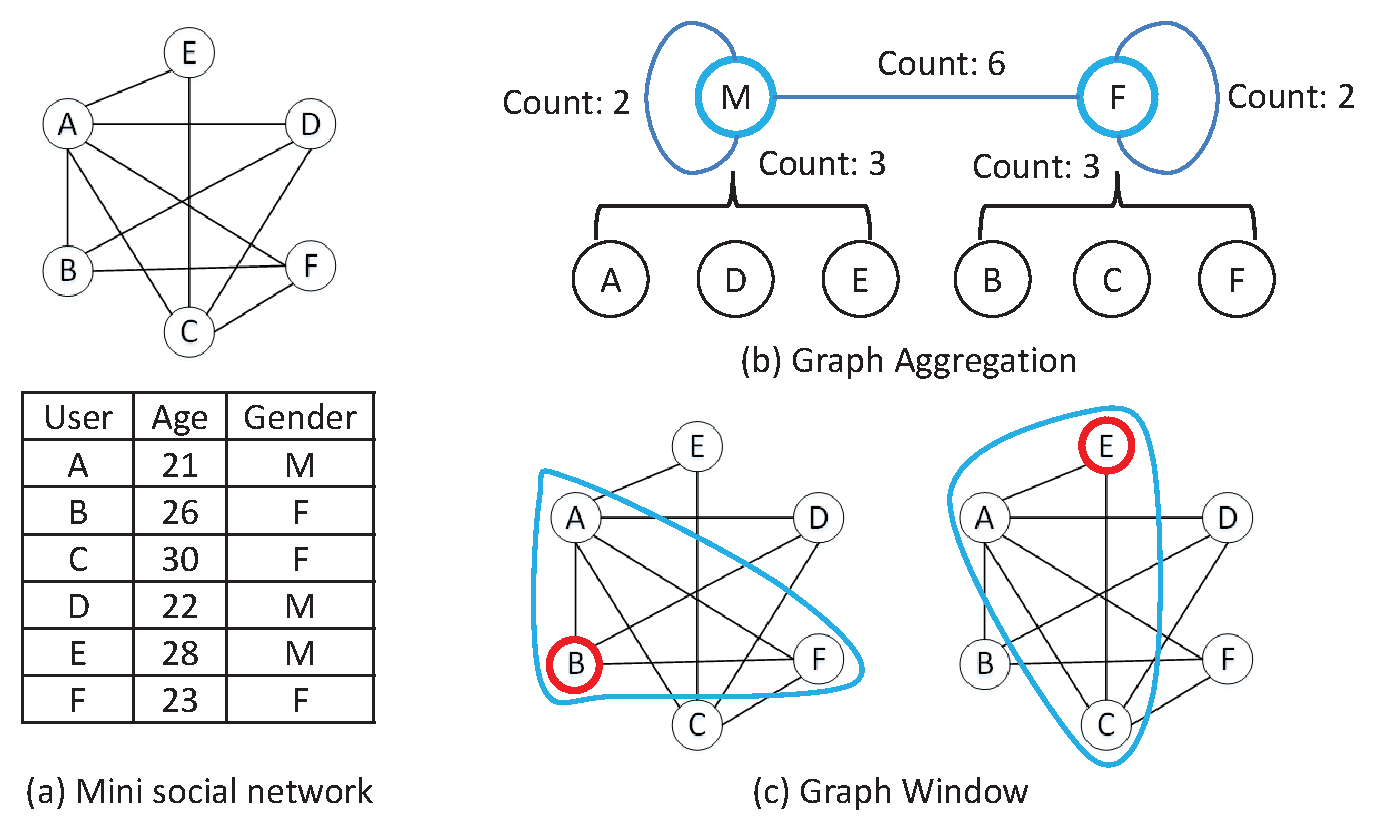
\includegraphics[width=0.8\textwidth]{chapter2/graphagg-window}
\caption{Illustration of \emph{Graph Aggregation} and \emph{Graph Window Queries}. (a) is an example social network, (b) is graph aggregation, (c) are the windows of vertexes $B$ and $E$.}
\label{fig:rw-agg-window}
\end{figure}

%Traditional graph data analytics focus on
%graph OnLine Analytic Processing (OLAP)~\cite{zhao2011graph,wang2014pagrol,chen2008graph,tian2008efficient},
%which is different from Graph Window Queries.
%In a general model, graph OLAP applies analytics on each partition
%of the graph, where the partitions are created based on some
%attribute values of vertexes or edges. On the other hand, graph
%window queries aim to find the subgraph associated with each vertex
%and compute analytics over each subgraphs. Indeed, such differences also arise in the relational context, where different 
%techniques are developed to evaluate OLAP and window function queries.


%In graph OLAP, information 
%in a graph is summarized by partitioning the graph's nodes/edges (based on some attribute values) 
%and computing aggregate values from each partition.
%Graph window queries, on the other hand, compute aggregate values for each graph node w.r.t. 
%the subgraph associated with the node.
%Indeed, such differences also arise in the relational context, where different 
%techniques are developed to evaluate OLAP and window function queries.
%
%
%GWFs are also different from graph aggregation \cite{zhao2011graph,wang2014pagrol,chen2008graph,tian2008efficient} in graph OLAP.
%In graph OLAP, information in a graph are summarized
%by partitioning the graph's nodes/edges (based on some attribute values) and computing aggregate values for each partition.
%GWFs, on the other hand, compute aggregate values for each graph node w.r.t. the subgraph associated with the node.
%Indeed, such differences also arise in the relational context, where different 
%techniques are developed to evaluate OLAP and window function queries.

\subsection{Reachability Queries and Indexes}
Classic reachability queries, which
answer whether two vertexes are connected, have 
been studied extensively in literature. 
To facilitate fast query processing, many indexes are
proposed~\cite{cheng2013tf,cheng2012k,wei2014reachability,yu2010graph}. 
Although our graph window queries
can be built on top of the reachability queries, directly
using these techniques is inefficient. For example, the
most related reachability
query to our $k$-hop window query is the $k$-reach query~\cite{cheng2012k} which
tests if an input pair of vertexes is within a $k$-hop distance. In order
to compute the $k$-hop window query for $n$ vertexes, there would be $\theta(n^2)$
reachability tests. This would be inefficient on graphs
with over millions of vertexes.

%
%Reachability queries, 
%asking if two vertexes are connected, are important 
%in supporting many useful analytics. 
%Indexing techniques have been proposed to 
%efficiently determine whether an input pair of vertices is within a distance of k-hops (e.g. k-reach index \cite{cheng2012k}) or reachable (e.g. reachability index \cite{yu2010graph}). However, such techniques are not efficient for computing the k-hop window or topological window for a set of $n$ vertices with a time complexity of $O(n^2)$. 

\subsection{Top-$k$ Neighborhoods}
In \cite{yan2010top}, the authors investigated the problem of finding the vertexes
that have top-$k$ highest aggregate values over their $h$-hop neighbors.
This is similar to our $k$-hop query, while the difference is that they
focus on providing pruning techniques to select the $k$ best vertexes and our graph
window query aims to compute the analytics for each vertex. Therefore,
in our setting, the pruning techniques in~\cite{yan2010top} does not take effect
and would be equivalent to the non-indexed approach.% as described in Section~\ref{sec:graph:non-index}.
%This is similar to our $k$-hop queries while the difference is that they
%focus on providing pruning techniques to select $k$ best vertexes and our graph
%window query aims to compute the analytic values for each vertex. In our 
%setting, their techniques degrade to the non-index approach as described in Section~\ref{};

%
%They proposed mechanisms to prune the computation by using two properties: First, the locality between vertexes is used to propagate the upper-bound of aggregation; Second, the upper-bound value of aggregates can be estimated from the distribution of attribute values. However, all these pruning techniques are not applicable in our work, as we need to compute the aggregation value for every vertex. In such a scenario, techniques in \cite{yan2010top} degrade to the non-indexed approach as described in Section 4.

\subsection{Egocentric Networks}
Egocentric networks~\cite{ma2010ego,marsden2002egocentric} 
have been playing an important role in network study. The egocentric networks
refer to the neighborhood structure of each vertex
in a graph. Although many works have studied structural analysis on egocentric networks, they do not consider efficient processing 
of data analytics (e.g., aggregation) within each egocentric network. 
Recently, Jayanta et.al. \cite{mondal2014eagr} 
proposed an EAGR system to summarize attribute information among 
each vertex's neighborhoods. Their technique builds an overlay graph 
to leverage the shared components among vertexes' neighborhoods structures to
boost query processing.
%
% Their technique is to build an overlay graph to
%leverage the shared components among vertexes' neighborhoods structures.
%which can be 
%mined via Frequent-Pattern Mining Tree (FP-Tree). Then, an overlay graph is 
%constructed to record the shared components.
Technically, EAGR runs in iterations and starts with the vertex-neighborhood mapping
as the initial overlay graph. During each iteration,
it sorts vertexes in an overlay graph according to their neighborhood information. 
Then an FP-Tree~\cite{han2000mining} is built to mining the largest shared components based
on the sorted vertexes.
%Then the sorted vertexes 
%are split into equal-sized chunks. For each chunk, 
%a FP-Tree is built to mining the largest shared components. 
As the algorithm iterates, the overlay graph evolves to be sparser. 

%Since EAGR runs in multiple iterations, it requires
%to rebuilt the FP-Tree in every iterations.
%of an overlay graph where
%each 
%
%They use the Frequent-Pattern Tree heuristic~\cite{} 
%to find the shared components among each vertex's neighborhoods. 
%It starts by building an
%bipartite overlay graph to represent the vertex-neighbor mapping.
%Then it aims to
%find the bi-cliques in the overlay graph, where
%each bi-clique represents a set of vertexes whose neighborhood
%aggregates can be shared. Once a bi-clique is found, it is inserted back to the overlay graph as
%a virtual node to remove redundant edges. EAGR finds bi-cliques in iterations. During each iteration,
%it sorts each vertexes in overlay graph by their neighborhood information. Then the sorted vertices 
%are split into equal-sized chunks. For each chunk, it then builds a FP-Tree to mining the large bi-cliques. 
%As the algorithm iterates, the overlay graph evolves to be less dense. 
%

The main drawback of EAGR is its high demands of resources 
on the overlay construction. In terms of memory cost, EAGR assumes the 
initial vertex-neighbor mapping can be stored in memory. However, the assumption does not scale well for computing higher hop windows (such as k $\geq 2$). 
For instance, a LiveJournal social network graph \footnote{Available at http://snap.stanford.edu/data/index.html, which is used \cite{mondal2014eagr}} (4.8M nodes, 69M edges) generates over 100GB mapping information for k=2 in adjacency list 
representation. If the neighborhood information is resided in disk, the performance of EAGR will
largely reduced.  In terms of computational cost, EAGR requires to sort all vertexes 
in a graph and build an FP-Tree in each iteration. When the graph has
millions of vertexes, the construction of the index is largely slow down.

%It requires the neighborhood information to be pre-computed, which is then used in the sorting phase of each iteration. In EAGR, the neighborhood information is assumed to be stored in memory.
%However, the assumption does not scale well for computing higher hop windows (such as k $\geq 2$). 
%For instance, a LiveJournal social network graph \footnote{Available at http://snap.stanford.edu/data/index.html, which is used \cite{mondal2014eagr}} (4.8M nodes, 69M edges) generates over 100GB mapping information for k=2 in adjacency list 
%representation. If the neighborhood information is resided in disk, the performance of EAGR will
%largely reduced. Similarly, if the neighborhood information is computed on-the-fly, EAGR needs
%to perform the computation in each iteration, which largely increases indexing time. 

We tackle these drawbacks by adopting a hashing based approach that clusters each vertex according to
its neighborhood similarity. During the hashing, a vertex's neighborhood information
is computed on-the-fly. As compared to the sorting based approach, we do not require vertex's neighborhood
to be resided in memory. 
In order to reduce the repetitive computation, we adopt a Dense Block heuristic to leverage
the shared components among vertexes' neighborhoods. We then propose an estimation scheme that
further reduces the number of neighborhood accesses.
%To further reduce the neighborhood access, we propose an estimated indexing construction algorithm that only requires a vertex's smaller-hop neighborhood to be computed during clustering. 
Experiments show that our schemes outperform EARG in both query processing and memory usage. 
Our methods are able to perform well even when EAGR algorithm fails when neighborhood information overwhelms system's memory, and our methods takes much shorter indexing time.
%
% As shown in Section~\ref{sec:graph:experiment}, our proposed mesthods 
%is able to perform well even when EAGR algorithm fails when neighborhood information overwhelms system's memory.
%To further reduce the neighborhood access, we adapted a Dense Block heuristic to process each vertex
%in one pass. 
%Experiments shows that the query performance of our heuristic is comparable to EAGR's, but with
%much shorter indexing time.
  

%Window function was proposed in \cite{zemke2012s}, which is widely used in SQL data analytic. There are several optimization on standard window functions \cite{cao2012optimization, bellamkonda2013adaptive}. \cite{cao2012optimization} optimize window function via shared sorted components, and \cite{bellamkonda2013adaptive} optimized window function via partition. However, in \emph{GWF}, the sorting and partition is no longer required, thus their techniques are not applicable in the graph window context.
%\remark{We haven't mention GWFs in introduction section, does this needs to be mentioned?}
\eat{Our proposed graph window functions (GWFs) for graph databases is inspired by the usefulness of window functions in relational analytic queries
\cite{zemke2012s}.

A window function in SQL typically specifies a set of partitioning attributes $A$ and an aggregation function $f$.
Its evaluation first partitions the input records based on $A$ to compute $f$ for each partition,
and each input record is then associated with the aggregate value corresponding to the partition that contains the record.
Several optimization techniques \cite{cao2012optimization, bellamkonda2013adaptive}
have also been developed to evaluate complex SQL queries involving multiple window functions.
%by reducing the overall partitioning cost to evaluate the aggregation functions.
%\remark{Need to also cite an earlier Oracle tech report.}

%However, in \emph{GWF}, the sorting and partition is no longer required, thus their techniques are not applicable in the graph window context.
However, the semantics and evaluation of window functions are very different between relational and graph contexts.
Specifically, the partitions (i.e., subgraphs) associated with GWFs are not necessarily disjoint; thus,
the evaluation techniques developed for relational context \cite{cao2012optimization, bellamkonda2013adaptive} are not applicable to GWFs. %\remark{\cite{bellamkonda2013adaptive} focuses on utilizing partition to parallel window processing, and \cite{cao2012optimization} focuses on leveraging sorting among windows. However sorting and partitioning are no longer exists in GWFS, thus, their work are not applicable}

GWFs are also different from graph aggregation \cite{zhao2011graph,wang2014pagrol,chen2008graph,tian2008efficient} in graph OLAP.
In graph OLAP, information in a graph are summarized
by partitioning the graph's nodes/edges (based on some attribute values) and computing aggregate values for each partition.
GWFs, on the other hand, compute aggregate values for each graph node w.r.t. the subgraph associated with the node.
Indeed, such differences also arise in the relational context, where different 
techniques are developed to evaluate OLAP and window function queries.

In \cite{yan2010top}, the authors investigated the problem of finding the vertices that have top-k highest aggregate values over their h-hop neighbors. They proposed mechanisms to prune the computation by using two properties: First, the locality between vertices is used to propagate the upper-bound of aggregation; Second, the upper-bound value of aggregates can be estimated from the distribution of attribute values. However, all these pruning techniques are not applicable in our work, as we need to compute the aggregation value for every vertex. In such a scenario, techniques in \cite{yan2010top} degrade to the non-indexed approach as described in Section 4.
%rather than finding the top-k values.  

%\cite{cheng2012k} provided a \emph{K-Reach} index for fast determining whether two vertices can be reached within K-hop distance. However, \emph{K-Reach} index can not be directly used to support the k-hop window query due to its high overhead. Gathering the window of one vertex may involve $|V|$ reachability detections which results in the complexity of $O(|V|^2)$ to compute the windows for all the vertices, where $|V|$ is the number of vertices.}  

Indexing techniques have been proposed to efficiently determine whether an input pair of vertices is within a distance of k-hops (e.g. k-reach index \cite{cheng2012k}) or reachable (e.g. reachability index \cite{yu2010graph}). However, such techniques are not efficient for computing the k-hop window or topological window for a set of $n$ vertices with a time complexity of $O(n^2)$. 



%Indexing techniques \cite{yu2010graph,cheng2012k} is able to test whether a vertex belongs to another vertex's window. \cite{cheng2012k} proposed \emph{K-Reach} index which tests a whether an input pair of vertices is within a distance of k-hops, thus it can be used to compute \emph{k-hop} window. \cite{yu2010graph} surveys a wealth of \emph{Reachability Indices} which tests whether a input pair of vertices is reachable, thus it can be used to compute \emph{topological} window. However, those techniques are not efficient for computing either \emph{k-hop} or \emph{topological} window, since for a set of $n$ vertices, their complexity of forming window is of $O(n^2)$.

% which efficiently determines whether an input pair of vertices is within a distance of k-hops. Thus \emph{K-Reach} is able to facilitate \emph{k-hop} window. While, \cite{yu2010graph} presents a survey of reachability indices which determine whether an input pair of vertices is connected. Thus, those techniques is able to facilitate \emph{topological} window. However, such techniques are not efficient for computing either \emph{k-hop} or \emph{topological} window, since for a set of $n$ vertices, their complexity of forming window is of $O(n^2)$.

%Indexing techniques such as the \emph{K-Reach} index \cite{cheng2012k} have been proposed
%to efficiently determine whether an input pair of vertices is within a distance of k-hops.  
%However, such techniques are not efficient for computing the k-hop window for a set of $n$ vertices has a time complexity of $O(n^2)$.

%However, \emph{K-Reach} index can not be directly used to support the k-hop window query due to its high overhead. Gathering the window of one vertex may involve $|V|$ reachability detections which results in the complexity of $O(|V|^2)$ to compute the windows for all the vertices, where $|V|$ is the number of vertices.}  
%
%use \emph{K-Reach} index to collect the windows of each vertex 
%
%it incurs high overhead to adopt \emph{K-Reach} index to gather the window for a k-hop window query. The reason is that  
%
%is unable to answer k-hop window query. To see this, for each vertex, $|V|$ reachability queries need to be performed in order to gather a window. The total running time of this approach is $O(|V|^2|R|)$, where $|R|$ is the cost for answering one reachability query. This is obvious not acceptable in terms of query performance.

\eat{\cite{mondal2014eagr} proposed an EAGR system which evaluates neighborhood-based aggregation
queries over low hops (k = 1). They follow a in-memory model and assume the k-hop information 
for each vertex is pre-computed. Based on the neighborhood information, it first sort each vertex
using lexicographic order. Then vertices are split into equal sized chunks. For each chunk, it 
then builds a Frequent-Pattern Tree for iteratively mining the shared components between each vertex's 
neighborhoods. Lastly, it builds an overlay graph based on the shared components for efficient computing.
}

\cite{mondal2014eagr} proposed an EAGR system, which uses the famous VNM heuristic and Frequent-Pattern
Tree to find the shared component among each vertex's neighborhoods. It starts by building an
overlay graph as a bipartite graph representing the vertex-neighbor mapping. Then it aims to
find the bi-cliques in the overlay graph. Each bi-clique represents a set of vertices whose neighborhood
aggregates can be shared. Once a bi-clique is found, it is inserted back to the overlay graph as
a virtual node to remove redundant edges. EAGR find bicliques in iterations. During each iteration,
it sorts each vertices in overlay graph by their neighborhood information. Then the sorted vertices 
are split into equal-sized chunks. For each chunk, it then builds a FP-Tree to mining the large bi-cliques. 
As the algorithm iterates, the overlay graph evolves to be less dense. 


The main drawback of EAGR is its demands of high memory usage on overlay construction. It
requires the neighborhood information to be pre-computed, which is used in the sorting phase
of each iteration. In EAGR the neighborhood information is assumed to be stored in memory.
However, the assumption does not scale well for computing higher hop windows (such as k $\geq 2$). 
For instance, a LiveJournal social network graph \footnote{Available at http://snap.stanford.edu/data/index.html, which is used \cite{mondal2014eagr}} (4.8M nodes, 69M edges) generates over 100GB mapping information for k=2 in adjacency list 
representation. If the neighborhood information is resided in disk, the performance of EAGR will
largely reduced. Similarly, if the neighborhood information is computed on-the-fly, EAGR needs
to perform the computation in each iteration, which largely increases indexing time.

We tackle this drawback by adapting a hashing based approach that clusters each vertex according to
 its neighborhood similarity. During the hashing, the vertex's neighborhood information
is computed on-the-fly. As compared to sorting based approach, we do not require vertex's neighborhood
to be pre-reside in memory. In order to reduce the repetitive computation of vertex's neighborhood,
we further propose an estimation based indexing construction algorithm that only require a vertex's small
hop neighborhood to be computed during clustering. As our experiments show, our proposed methods 
can perform well even when EAGR algorithm fails when neighborhood information overwhelms system's memory.
To further reduce the neighborhood access, we adapted a Dense Block heuristic process each vertex
in one pass. Experiments shows that the performance of our heuristic is comparable to EAGR's, but with
much shorter indexing time.
  


  

%
%\eat{The work that is most related to ours is 
% \cite{mondal2014eagr} - referred as EAGR 
%which examines the evaluation of neighborhood-based or ego-centric (similar to our k-hop window)
%aggregation queries. 
%Both EAGR and our DBIndex aim to speed up the aggregation computation by sharing the processing of the intersections among different windows. There are, however, two main differences between our work and EAGR.
%First, while both EAGR and our approach are main-memory techniques, 
%our approach is much more memory efficient and scalable than EAGR.
%%which results in a high scalablity to support large-scale graphs. 
%%The scalability limitation of EAGR arises due to its assumption that the mapping information about all vertices' windows must be precomputed and stored in main memory, and memory-inefficient data structure, Frequent Pattern Tree (FPT) adopted to construct the overlay graph. Note that FPT has almost the same high space requirement as the mapping information for a large k: for k-hop queries, in $O(|V|d^k)$ if represented as an adjacency lists and
%The scalability limitation of EAGR arises due to its large memory requirement 
%for both the mapping information for all vertex windows 
%as well as a Frequent Pattern Tree (FPT) data structure used to construct an overlay graph. 
%Each of these main-memory structures
%has a space complexity of $O(nd^k)$ if represented as an adjacency lists and
%$O(n^2)$ if represented as adjacency matrix,
%for $k$-hop queries where $n$ denotes the number of vertices and $d$ denotes the average node degree. 
%For instance, a LiveJournal social network graph \footnote{Available at http://snap.stanford.edu/data/index.html, which is used \cite{mondal2014eagr}} (4.8M nodes, 69M edges) generates over 100GB mapping information for k=2 in adjacency list representation; the size is even larger if a matrix representation is used. 
%In contrast to EAGR, our approach is more scalable as it does not require the existence of the large mapping and data structure, and thus is more memory efficient. The peak memory usage for our algorithm is only around 8GB for such a large graph. 
%Second, we formally define and propose a new type of query, topological window query and a new index I-Index, which are not covered in \cite{mondal2014eagr}. 
%}


%unlike our work, EAGR does not consider topological window queries.
%While topological queries could be evaluated as a form of k-hop queries 
%(by treating a node's topological neighborhood as its k-hop neighborhood),
%we show that topological queries could be evaluated more efficiently using specialized techniques that take into account of the 
%topological properties. 




%EAGR further assumes that the information about each node's window, referred as the {\em mapping information}, has been precomputed
%and stored in the main memory.
%Based on the mapping information, EAGR further computes an index structure (known as overlay graph) in multiple iterations where each iteration builds one Frequent Pattern  (FP) Tree to construct the overlay graph. Note that the size of the FPTree is essentially the same as the mapping information.  
%For $k$-hop queries, the space requirement for the mapping information could be very large for a large $k$:
%$O(|V|d^k)$  if represented as an adjacency lists and
%$O(|V|^2)$  if represented as adjacency matrix,
%where $|V|$ denotes the number of graph vertices and $d$ denotes the average node degree. Under this high complexity, a LiveJournal social network graph \footnote{Available at http://snap.stanford.edu/data/index.html, which is used \cite{mondal2014eagr}} (4.8M nodes, 69M edges) generates over 100GB vertex-window mapping under 2-hop scenario in adjacency list representation. This size is even larger in a matrix representation due to the $O(|V|^2)$ space complexity of matrix.  The assumption of in-memory mapping limits the scalability of EAGR with respect to the number of hops. In contrast to EAGR, our approach is more scalable as it does not require the existence of the large mapping and thus is more memory efficient. The peak memory usage for our algorithm is only around 8GB for such large graph. 
%Second, unlike our work, EAGR does not consider topological window queries.
%While topological queries could be evaluated as a form of k-hop queries 
%(by treating a node's topological neighborhood as its k-hop neighborhood),
%we show that topological queries could be evaluated more efficiently using specialized techniques that take into account of the 
%topological properties. We emphasize that our index can be directly used to handle dynamic graphs when the attribute changes as EAGR did. However, it is non-trivial to support structure changes. In EAGR, this was 
%briefly discussed  without any experimental evaluation. We intend to study how to efficiently update indices in the presence of structural data updates as part of our future work. %%%we add this last point is to say why we dont study the dynamic graphs.  


%The work that is most related to ours is 
% \cite{mondal2014eagr} 
%which examines the evaluation of continuous k-hop window (referred to as neighborhood-based or ego-centric) 
%aggregation queries for dynamic graphs (i.e., in the presence of dynamic updates to the graph structure/attribute values). 
%In [7], a scheme called EAGR is proposed to process these queries. Both EAGR and our work aim to speed up the aggregation computation by sharing the processing of the intersections among different windows. There are, however, two main differences between our work and EAGR.
%First, while both EAGR and our approach are main-memory techniques,
%which assume that the data graph fits in main memory,
%EAGR further assumes that the information about each node's window, referred as the {\em mapping information}, has been precomputed
%and stored in the main memory.
%Based on the mapping information, EAGR further computes an index structure (known as overlay graph) in multiple iterations where each iteration builds one Frequent Pattern  (FP) Tree to construct the overlay graph. Note that the size of the FPTree is essentially the same as the mapping information.  
%For $k$-hop queries, the space requirement for the mapping information could be very large for a large $k$:
%$O(|V|d^k)$  if represented as an adjacency lists and
%$O(|V|^2)$  if represented as adjacency matrix,
%where $|V|$ denotes the number of graph vertices and $d$ denotes the average node degree. Under this high complexity, a LiveJournal social network graph \footnote{Available at http://snap.stanford.edu/data/index.html, which is used \cite{mondal2014eagr}} (4.8M nodes, 69M edges) generates over 100GB vertex-window mapping under 2-hop scenario in adjacency list representation. This size is even larger in a matrix representation due to the $O(|V|^2)$ space complexity of matrix.  The assumption of in-memory mapping limits the scalability of EAGR with respect to the number of hops. In contrast to EAGR, our approach is more scalable as it does not require the existence of the large mapping and thus is more memory efficient. The peak memory usage for our algorithm is only around 8GB for such large graph. 
%Second, unlike our work, EAGR does not consider topological window queries.
%While topological queries could be evaluated as a form of k-hop queries 
%(by treating a node's topological neighborhood as its k-hop neighborhood),
%we show that topological queries could be evaluated more efficiently using specialized techniques that take into account of the 
%topological properties. We emphasize that our index can be directly used to handle dynamic graphs when the attribute changes as EAGR did. However, it is non-trivial to support structure changes. In EAGR, this was 
%briefly discussed  without any experimental evaluation. We intend to study how to efficiently update indices in the presence of structural data updates as part of our future work.

%%{I added these aspects because Prof Yan mentioned about this point in the TAC meeting}
%Our \emph{DB-Index} and \emph{I-Index} effectively compress the vertex-window mapping, which is conceptually similar to graph compression \cite{Fan2012QPG,Grabowski2014TSW,Toivonen2011CWG,Buehrer2008SPM:}. However, these techniques fail to work in our scenario, since they do not consider aggregation query preservation and they assume initial vertex-mapping is memory-resides.
}
\section{$k$-Sketch Query}\label{sec:related_work}
Our proposed $k$-Sketch query is closely related
to three areas: automatic news detection, frequent episode mining and top-$k$ diversity query.

\subsection{Automatic News Detection}
An prominent usage of $k$-Sketch query is on Computational
Journalism where pioneer works include the 

Earlier works on automatic news theme generation were focused on finding interesting themes from a single event. For example, Sultana et al.~\cite{sultana2014incremental} proposed the \emph{Situational Fact} pattern, which is modeled as a skyline point under certain dimensions. Wu et al.~\cite{wu2012one} proposed the \emph{One-of-the-Few} concept to detect news themes with some rarities. Examples of candidate news themes for the above two patterns are illustrated in Table~\ref{tbl:related_works}.

{\renewcommand{\arraystretch}{1.2} 
\begin{table}[h]
\centering
\begin{tabular}{|l|l|}
\hline
\textbf{Method} & \textbf{Example news theme}\\
\hline
Situational facts~\cite{sultana2014incremental} & \pbox{22cm}{\vspace{.3\baselineskip} Ellen's tweet generates 3.3M retweets\\ with 170,000 comments.\vspace{.3\baselineskip}} \\
\hline
One-of-the-few facts~\cite{wu2012one} & \pbox{22cm}{\vspace{.3\baselineskip}Perry is one of the three candidates \\  who received \$600k\vspace{.3\baselineskip}} \\
\hline
Prominent streak~\cite{zhang2014discovering} & Kobe scored 40+ in 9 straight games!  \\
\hline
Rank-aware theme & \pbox{22cm}{\vspace{.3\baselineskip}Kobe scored 40+ in 9 straight games\\ ranked 4th in NBA history!\vspace{.3\baselineskip}} \\
\hline
\end{tabular}
\caption{Examples of different news themes}
\label{tbl:related_works}
\end{table}
}

Zhang et al.\cite{zhang2014discovering} proposed using prominent streak to generate interesting news themes.
In \cite{zhang2014discovering}, a \emph{Prominent Streak} is characterized by a 2D point which represents the window length and the minimum value of all events in the window. The objective is to discover the non-dominated event windows for each subject, where the dominance relationship is defined among streaks of the same subject. Our model differs from \cite{zhang2014discovering} in two aspects. First, we look at the global prominence (quantified by the rank) among all subjects rather than local prominence (quantified by the dominance) within one subject. Second, our model provides the best $k$-sketch for each subject whereas \cite{zhang2014discovering} returns a dominating set which could be potentially large. 
 
\subsection{Frequent Episode Mining}
In time sequenced data mining, an episode~\cite{mannila1997discepisodes,
zhou2010serialepisodes, tatti2012strictepisodes, laxman2007nonoverlapepisodes} is 
defined as a collection of time sequenced events which occur together within a time window. The uniqueness of an episode is determined by the contained events. The objective is to discover episodes whose 
occurrences exceeding a support threshold. 
Our sketch discovery differs from the episode mining in three major aspects. First, an episode is associated with a categorical value while our sketch is defined on numerical values. Second, the episodes are selected based on the occurrence, while in sketch, news themes are generated in a rank-aware manner. Finally, episode mining does not restrict its output size, while sketch only outputs the best $k$ news themes. As such, episode mining techniques cannot be straightforwardly applied to sketch discovery.

%First, episode concerns event types (alphabets), while streak concerns the analytic values. The mismatch makes episode mining inappropriate for sketch discovery since counting the occurrence based on analytic values is not meaningful. Second, candidate episode is selected based on the number of occurrence compared to a threshold, whereas candidate streak is based on the rank among other streaks with the same window size. The notion of rank does not straightforwardly apply to episodes thus making the problem different from sketch discovery. Third, in sketch discovery, we aim to find the best $k$ streaks, while in episode mining, there is no evaluation among episodes thus it does not fit the needs of sketch discovery.


\subsection{Top-$k$ Diversity Query}
Top-$k$ diversity queries~\cite{agrawal2009diversifying,borodin2012max,drosou2014diverse,chen2015diversity}
aim to find a subset of objects to maximize a scoring function. The scoring function normally penalizes
a subset if it contains similar elements. Our sketch discovery problem has two important distinctions
 against the top-$k$ diversity queries.
First, the inputs of the scoring function are known in advance in top-$k$ diversity queries; whereas in our problem, the ranks of event windows are unknown. Since their calculations are expensive, we need to devise efficient methods to compute the ranks.
Second, existing methods for online diversity queries~\cite{borodin2012max,drosou2014diverse,chen2015diversity} only study
the update on a single result set when a new event arrives. However our online sketch maintenance 
incurs the problem of multiple sketch updates for each new event. Such a complex update pattern has not been studied yet and hence there is a need to develop efficient update scheme.

%Recently, Chen et al.~\cite{chen2015diversity} studied the diversity-aware top-k publish/subscribe for text stream.  
%Users subscribe text contents by 
%issuing queries with keywords. Whenever a document arrives, the matching subscriptions will include such document 
%if the inclusion of which leads to a better value of the ranking function defined. 
%However the methods proposed in~\cite{chen2015diversity} cannot be applied to our sketch discovery due to the 
%rank-aware feature of sketches. In our case, the sketches can still be affected
%even when news candidates associated with an arrival event are not inserted to any subject's sketch. However, in ~\cite{chen2015diversity}, an incoming document will be either inserted to the results of some subscriptions or simply discarded. Thus a novel solution must be devised to handle the complex update pattern of sketch monitoring. 


%Top-$k$ Diversity Query was proposed in~\cite{agrawal2009diversifying} in the information retrieval field
%and has attracted huge amount of research attentions recently~\cite{angel2011efficient, chen2015diversity,huang2015top}.
%In general, diversity-aware queries aim to find a subset of objects from the universal set
%to maximize a scoring function. Such scoring function will penalize a subset if it contains similar objects.
%One example is the maximum set coverage problem where the scoring function is the number of elements covered by a set of $k$ subsets.
%Our sketch discovery problem has two
%unique differences against the top-$k$ diversity problems.
%First, in diversity queries, the inputs of the scoring function are known in advance, e.g., the elements covered by each subset;
%whereas in sketch discovery the rank of each event window is unknown and expensive to compute. This motivates us to devise efficient
%methods to compute the ranks.
%Second, existing online diversity queries~\cite{borodin2012max,drosou2014diverse,chen2015diversity} only study efficient update on a single
%diverse set when an event arrives. However our online sketch monitoring incurs the problem of multiple sketches update
%for each new event. Such complex update patterns have not been studied yet and thus we propose an efficient update scheme.
%
%Recently, Chen et al.~\cite{chen2015diversity} studied the diversity-aware top-k publish/subscribe for text stream.  
%Users subscribe text contents by 
%issuing queries with keywords. Whenever a document arrives, the matching subscriptions will include such document 
%if the inclusion of which leads to a better value of the ranking function defined. 
%However the methods proposed in~\cite{chen2015diversity} cannot be applied to our online sketch monitoring due to the 
%rank-aware feature of sketches. In our case, the sketches can still be affected
%even when news candidates associated with an arrival event are not inserted to any subject's sketch. However, in ~\cite{chen2015diversity}, 
% an incoming document will be either inserted to the results of some subscriptions or simply discarded. 
%Thus a novel solution must be devised to handle the complex update pattern of sketch monitoring. 



\section{Movement Pattern Discovery Query}
\label{sec:related_works}
Related works can be grouped into three categories: \emph{co-movement patterns},
\emph{dynamic moving patterns} and \emph{trajectory mining frameworks}.
%The \emph{co-movement patterns} in literature consist 
%of five members, namely \emph{group}~\cite{wang2006grouppattern}, \emph{flock}~\cite{gudmundsson2004flock},
%\emph{convoy}~\cite{jeung2008convoy}, \emph{swarm}~\cite{li2010swarm} and \emph{platoon}~\cite{li2015platoon}.
%We have demonstrated the semantics of these patterns in Table~\ref{tbl:existing_co_patterns} and Figure~\ref{fig:related_work}. 
In this section, we distinguish the parallel GCMP mining from these concepts.
%In this section, we focus on comparing the techniques used in these works.
%For more trajectory patterns other than \emph{co-movement patterns}, 
%interested readers may move to~\cite{zheng2015survey} for a comprehensive survey.


\subsection{Flock and Convoy}
The difference between \emph{flock} and \emph{convoy} lies 
in the object clustering methods. In \emph{flock},
objects are clustered based on their distances. Specifically, the
objects in the same cluster need to have a pair-wised distance less than \emph{min\_dist}. 
This essentially requires the objects to be within a disk-region of delimiter less than \emph{min\_dist}.
In contrast, \emph{convoy} clusters objects using density-based spatial clustering~\cite{ester1996density}.
Technically, \emph{flock} utilizes a $m^{th}$-order Voronoi diagram~\cite{laube2005finding} to detect whether
a subset of object with size greater than $m$ stays in a disk-region. \emph{Convoy} employs
a trajectory simplification~\cite{douglas1973linesimplification} technique to boost pairwise distance computations in
the density-based clustering.
After clustering, both \emph{flock} and \emph{convoy} use a sequential scanning
method to examine each snapshots. During the scan, object
groups that appear in consecutive timestamps are detected. Meanwhile, the object groups that do not
match the consecutive constraint are pruned. 
However, such a method faces high complexity when supporting other patterns.
For instance, in \emph{swarm}, the candidate set during the sequential scanning grows
exponentially, and many candidates can only be pruned after the entire snapshots are scanned.

\subsection{Group, Swarm and Platoon}
Different from \emph{flock} and \emph{convoy}, all the \emph{group},\emph{swarm} and \emph{platoon}
patterns have more relaxed constraints on the pattern duration. Therefore, their techniques of mining are of
the same skeleton. The main idea of mining is to grow object set from an empty set
in a depth-first manner. During the growth, various pruning techniques are provided to prune 
unnecessary branches. \emph{Group} pattern uses a VG-graph to guide the pruning of false candidates~\cite{wang2006grouppattern}.
\emph{Swarm} designs two more pruning rules called backward pruning and forward pruning~\cite{li2010swarm}. \emph{Platoon}
further leverages a prefix table structure to steer the depth-first search. As shown by Li et.al.~\cite{li2015platoon},
\emph{platoon} outperforms other two methods in efficiency. 
However, the three patterns are not able to directly discover GCMPs.
Furthermore, their pruning rules heavily rely on the depth-first search nature, which lose their efficiencies
in the parallel scenario.

\subsection{Other Related Trajectory Patterns}
A closely related literature to co-movement patterns is the \emph{dynamic moving} patterns. Instead of requiring the same set of object traveling together, \emph{dynamic moving} patterns allow objects to temporally join or leave a group. Typical works include \emph{moving clusters}~\cite{kalnis2005movingclusters}, \emph{evolving convoy}~\cite{aung2010discovery}, \emph{gathering}~\cite{zheng2013gathering} etc. These works cannot model our GCMP since they enforce the global consecutiveness on the timestamps of a pattern. 

\subsection{Trajectory Mining Frameworks}
Jinno et al. in~\cite{jinno2012paralleltpattern} designed a MapReduce based algorithm to efficiently support \emph{T}-pattern discovery, where a \emph{T}-pattern is a set of objects visiting the same place at simliar time. Li et al. proposed a framework of processing online \emph{evolving group} pattern~\cite{li2013onlinegroup}, which focuses on supporting efficient updates of arriving objects. 
As these works essentially differ from co-movement pattern, their techniques cannot be directly applied to discover GCMPs.
